
\section{Performance-Analyse des derzeit fast durchgängig seriellen Codes}

\subsection{Datensets}
\begin{frame}{Datensets}
\textbf{Initialisierung:}
\begin{itemize}
	\item<2-> Detector Distortion
	\begin{itemize}
		\item ROI Größe: 1848x1848
		\item Gitterauflösung: 4
		\item Korrelationsgröße: 41
	\end{itemize}
\end{itemize}
\textbf{Hauptroutine:}
\begin{itemize}
	\item<3-> Experiment 6
	\begin{itemize}
		\item ROI Größe: 1450x1450 (Bild), 550x550 (Template)
		\item Gitterauflösung: 1
		\item Korrelationsgröße: 91
		\item unterschiedliche Pixelgröße
	\end{itemize}
	\item<4-> Lenses
	\begin{itemize}
		\item ROI Größe: 1450x1550 (Bild), 1450x1550 (Template)
		\item Gitterauflösung: 1
		\item Korrelationsgröße: 41
		\item gleiche Pixelgröße
	\end{itemize}
\end{itemize}
\end{frame}

\subsection{Gesamtlaufzeit}
\begin{frame}[allowframebreaks]
\frametitle{Gesamtlaufzeit}
%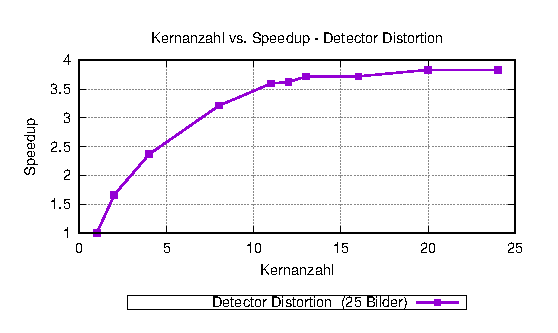
\includegraphics[width=0.9\linewidth]{img/times_detector_distortion}
\begin{center}
\scriptsize
Python 2.7, 2x Intel(R) Xeon(R) E5-2680 v3 (12 Kerne) @ 2.50GHz, kein MultiThreading
\end{center}
\framebreak
%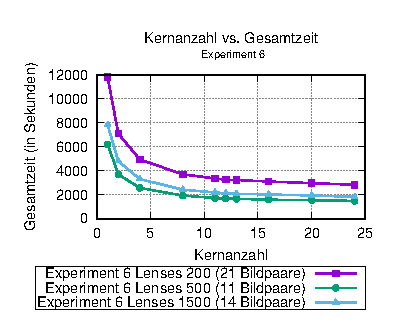
\includegraphics[width=0.9\linewidth]{img/times_exp6}
\begin{center}
\scriptsize
Python 2.7, 2x Intel(R) Xeon(R) E5-2680 v3 (12 Kerne) @ 2.50GHz, kein MultiThreading
\end{center}
\framebreak
%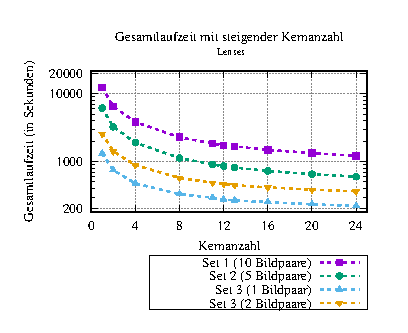
\includegraphics[width=0.9\linewidth]{img/times_lenses}
\begin{center}
\scriptsize
Python 2.7, 2x Intel(R) Xeon(R) E5-2680 v3 (12 Kerne) @ 2.50GHz, kein MultiThreading
\end{center}
\framebreak
\end{frame}

\subsection{Profiling}
\begin{frame}[allowframebreaks]
\frametitle{Profiling}
\begin{center}
%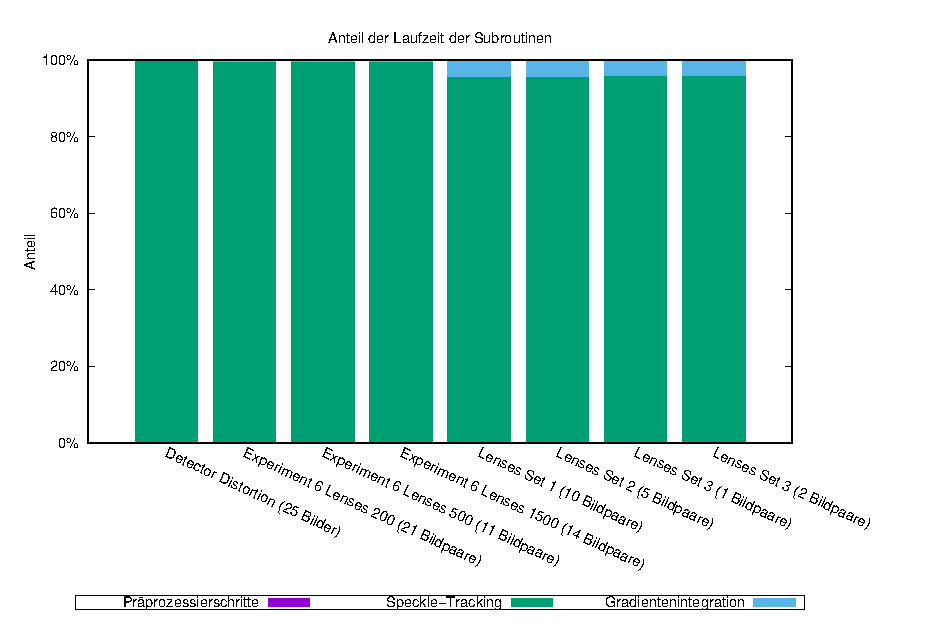
\includegraphics[width=0.74\linewidth]{img/main.eps}
%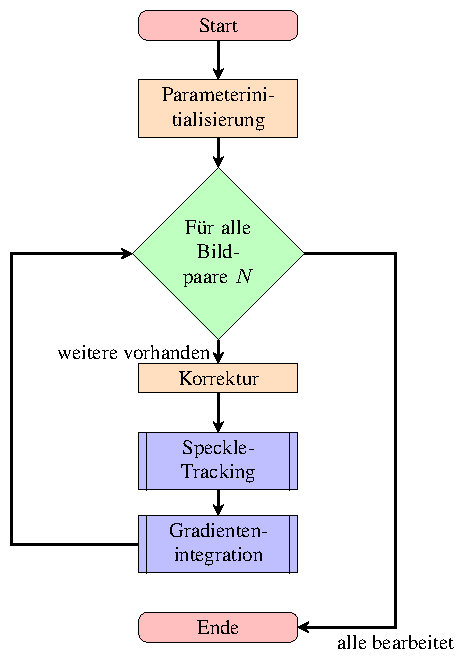
\includegraphics[width=0.25\linewidth]{tex/graph_main}
\framebreak

%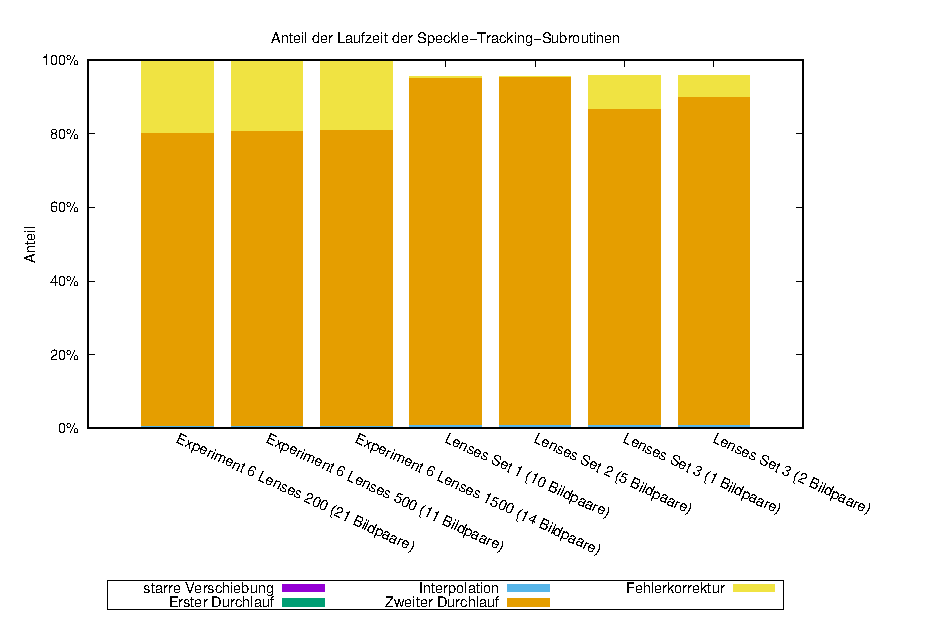
\includegraphics[width=0.84\linewidth]{img/speckle.eps}
%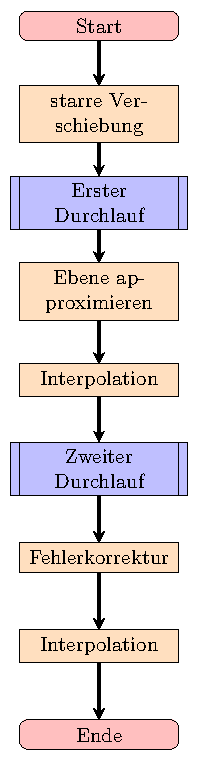
\includegraphics[width=0.15\linewidth]{tex/graph_speckle}

\framebreak

%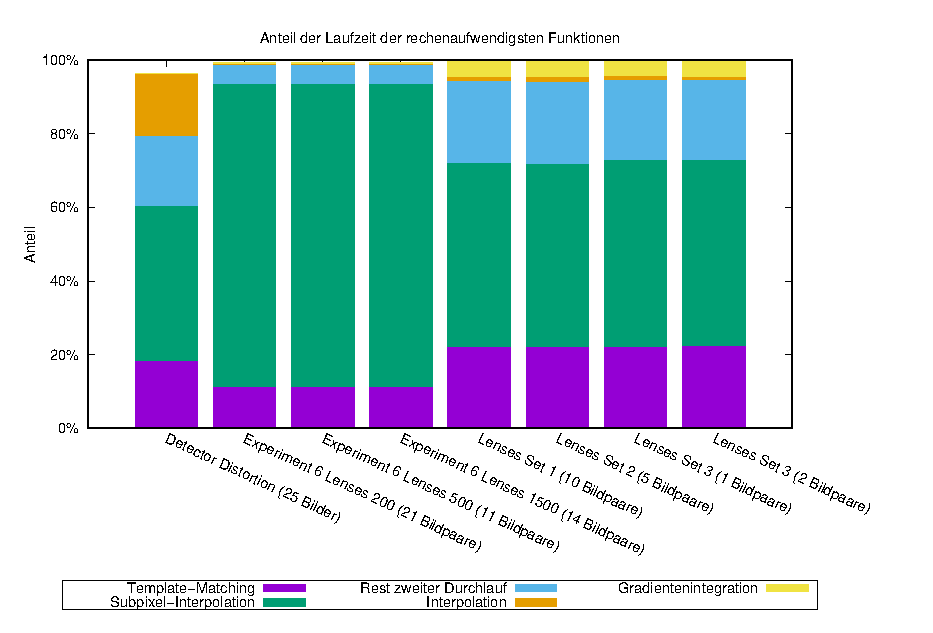
\includegraphics[width=0.94\linewidth]{img/slow.eps}\\
\textbf{$ \Rightarrow $ über 95\%}
\end{center}
\end{frame}
